\documentclass{standalone}
\usepackage{tikz}
\begin{document}
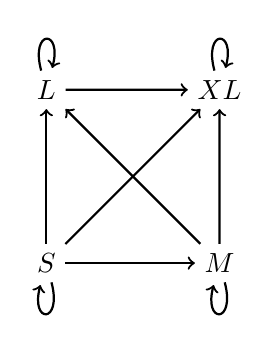
\begin{tikzpicture}[scale=1.1]
	\tikzset{arc lines/.style={thick,black, ->}}
	\node (S) at (0, 0) {$S$};
	\node (M) at (2, 0) {$M$};
	\node (L) at (0, 2) {$L$};
	\node (XL) at (2, 2) {$XL$};
	\draw [arc lines] (S) to (M);
	\draw [arc lines] (S) to (L);
	\draw [arc lines] (S) to (XL);
	\draw [arc lines] (M) to (L);
	\draw [arc lines] (M) to (XL);
	\draw [arc lines] (L) to (XL);
	\path [-stealth, thick]
	(S) edge [loop below] (S)
	(M) edge [loop below] (M)
	(L) edge [loop above] (L)
	(XL) edge [loop above] (XL)
	;
\end{tikzpicture}
\end{document}
